\chapter{Проектирование модели поведения виртуального агента}

В этом разделе описывается и обосновывается выбор инструментария для проектирования и программного воплощения 
модели поведения актора в заданной парадигме. Описываются ключевые моменты проектирования и программной реализации модели поведения актора.

\section{Описание предыдущей модели поведения актора и виртуального окружения}

В ходе выполнения программы записывались данные с оценками для первого и второго клоуна, а также с выводом сообщения совершенного 
действия, данные представлены на (Рис. \ref{pic:ris10}).

\begin{figure}[h]
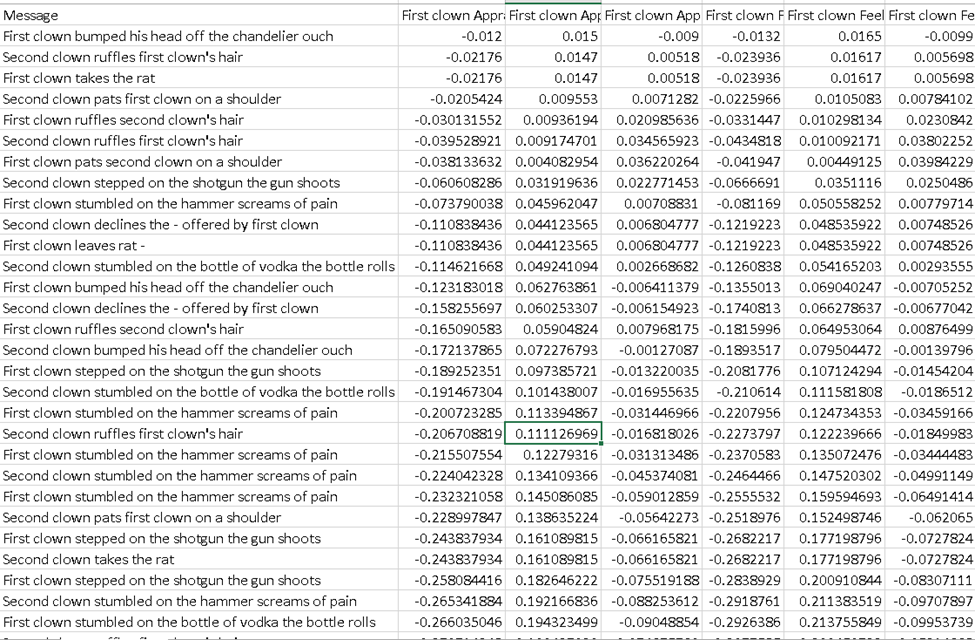
\includegraphics[width=0.75\columnwidth]{./img/ris10.png}
\centering
\caption{Оценки и действия совершенные первым виртуальным актором}
\label{pic:ris10}
\end{figure}

Для осуществления контроля за действиями акторов и их анализом система ведет записи в журнал событий. 
Журнал представляет собой текстовую таблицу. Записи выглядят следующим образом: каждая строка журнала соответствует своему событию, 
строка начинается с указания времени, когда была произведена запись. После указания времени указывается тип сообщения. 
Далее в сообщении показывается исполнитель действия, цель действия и номер действия из таблицы действий. 
После идет содержание сообщения, поясняющее произошедшее событие. После чего показаны оценки Appraisals и 
Feelings для доброжелательности, возбужденности и доминантности.

На (Рис. \ref{pic:ris11}) представлены гистограммы частот действий, совершаемых испытуемыми и модельным человеком.

\begin{figure}[h]
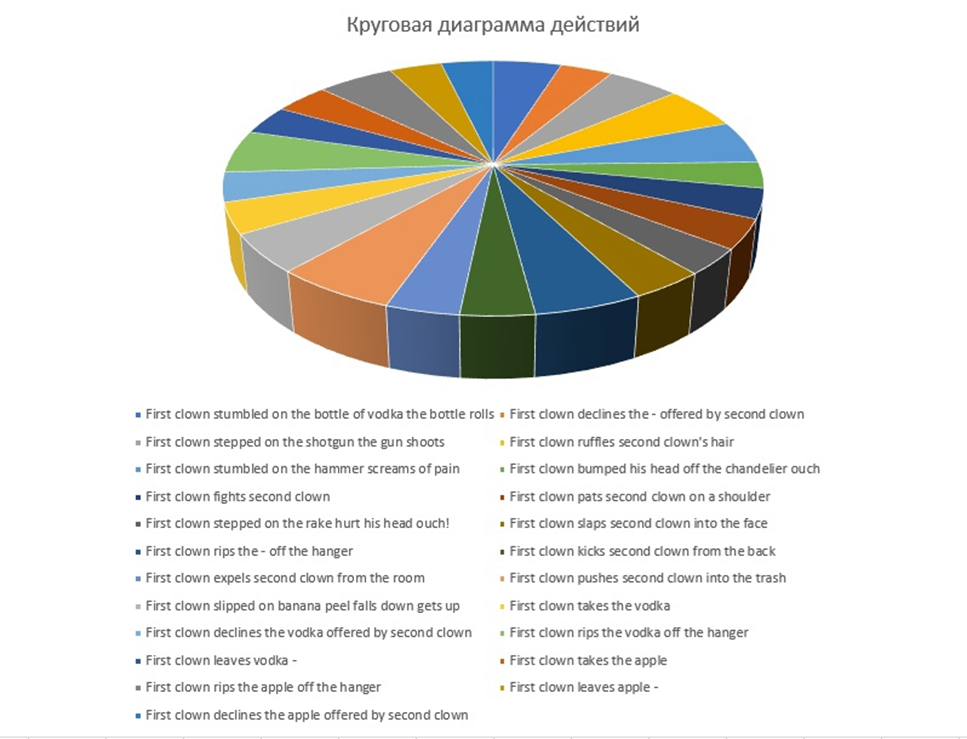
\includegraphics[width=0.75\columnwidth]{./img/ris11.png}
\centering
\caption{Диаграмма частот действий первого актора}
\label{pic:ris11}
\end{figure}

Исходя из диаграммы, можно заметить, что большое количество действий не использовалось. 
Данная ситуация возникла в ходе тестирования взаимодействия роботов с использованием моральной схемы, описанной в формуле \ref{eq:appraisals01}.

Существенным фактором, повлиявшим на работу моральной схемы, является оценка каждого действия отдельно по VAD, о чем говорися в работе \cite{Samsonovich02}. 
В ходе корректировки действий, основанной на опросе фокус группы, были произведены корректировки оценок. 
Результат корректировок виден на (Рис. \ref{pic:ris11}).

\section{Сбор данных, метрики и инструменты}

Для реализации сбора информации обычно используются следующие инструменты,  что отображено в работае \cite{parser01} :
\begin{itemize}
  \item	HTTP Client – клиент является библиотекой передачи, он находится на стороне клиента, отправляет и получает сообщения HTTP.
  \item	Beautiful Soup - это пакет Python для анализа документов HTML и XML. Он создает дерево синтаксического анализа для проанализированных страниц, которое можно использовать для извлечения данных из HTML, что полезно для парсинга веб-страниц.
  \item	Requests - это HTTP-библиотека для языка программирования Python. Цель проекта - сделать HTTP-запросы более простыми и удобными для человека.
  \item	AsyncIO – модуль, предназначенный для упрощения использования корутин и футур в асинхронном коде — чтобы код выглядел как синхронный, без коллбэков.
\end{itemize}

Основной принцип парсинга ресурсов для сбора информации осуществлялся при помощи написания алгоритмов на языке программирования Python. Для этого использовалась библиотека ButifulSoup, которая была выбрана для использования для чтения HTML, а также библиотека Requests, которая является стандартным инструментом для составления HTTP-запросов в Python. Простой и аккуратный API значительно облегчает трудоемкий процесс создания запросов. Таким образом, можно сосредоточиться на взаимодействии со службами и использовании данных в приложении. Так же из за большого количества реквестов было рационально использовать корутину, используя библиотеку Asyncio.

Такие HTTP методы, как GET и POST, определяют, какие действия будут выполнены при создании HTTP запроса. 
GET является одним из самых популярных HTTP методов. Метод GET указывает на то, что происходит попытка извлечь 
данные из определенного ресурса. Для того, чтобы выполнить запрос GET, используется requests.get(). 
Положительным ответом сервера является код 200. 

В метод requests.get() помещается URL, в которую может быть помещен JSON как текст запроса, либо при наличии 
API более упрощенный текстовый параметр, при наличии  токена как идентификатора аккаунта – токен.

response.status\_code, который равен 200, означает то что ответ от сервера получен положительный, 
текст запроса обработка, идентификация пользователя прошла успешна, возвращен ответ в формате JSON.

Иной же случай, когда нет доступа к API, оно платное либо его не существует. 
В таком случае скрипт будет выглядеть следующим образом.

В данном примере осуществляется request по URL, добавляется User-Agent, который имитирует пользователя, 
декодируются данные HTML в формат Unicode-8, который представляет собой распространённый стандарт 
кодирования символов, позволяющий более компактно хранить и передавать символы Юникода, используя 
переменное количество байт, и обеспечивающий полную обратную совместимость с 7-битной кодировкой ASCII.

Далее находим все классы таблиц и присваиваем переменным генератор, вытаскивающий 
из классов таблиц данные с соответствующим тегом.

С помощью BS4 можно найти в коде HTML все что требуется для создания нудного массива данных, 
далее для того, чтобы унифицировано хранить данные, следует использовать объектно-ориентированные форматы 
данных, такими бывают JSON и XML. JSON - текстовый формат обмена данными, основанный на JavaScript. 
Как и многие другие текстовые форматы, JSON легко читается людьми и в итоге был выбран как формат хранения данных в работе.

Для того чтобы спарсить сайт полностью и извлечь весь требуемый тип данных, используются рекурсивный подход. 
Для этого в работе используется пакет Python - html5lib, который реализует алгоритм парсинга HTML5, 
на который сильно влияют современные браузеры. Как только парсер получает нормализованную структуру 
содержимого, становится доступным поиск данных в любом дочернем элементе тега html. 
Искомые данные чаще всего находятся в теге “table”. После нахождения родительского тега, рекурсивно проходим по дочерним элементам. 
Для ссылок чаще всего используется тег “href”, далее из полученных ссылок извлекаем требуемый тип данных на сайте, в нашем случае это текст. 

Так как на сайте слишком много текста и достаточно большой процент содержания лишнего текста по типу маркировок, 
контекстной рекламы и прочего, ставится задача определения выявления значимого текста на сайте. 

Значимый текст выбирается на основании анализа его принадлежности к заранее определенным классам текста (или тематикам). 
Как правило, методы автоматической классификации основаны на методе машинного обучения: сначала получают 
обученную с помощью какого-либо алгоритма модель, качество которой определяет точность классификации. 
Таким образом, процесс обучения зависит от выбранного алгоритма и «чистоты» обучающей выборки, согласно работе о \cite{neural04}. 
Одним из фреймворков, который используется для того чтобы обучать модель по заранее определенным классам – это lingvo, 
реализованный для  .NET Framework, в котором используется Gradient Sign Dropout (GradDrop).

\section{Инструменты для анализа текста}

После сбора данных для их последующего использования в нейронной сети требуется осуществить разметку данных, для этого требуется 
выделить те слова определяющие какое-либо действие или предмет, которые будут семантически близки к заранее предопределенным 
типам действий или типам предметов.

Возможность идентификации семантической близости между словами сделала модель word2vec широко используемой в NLP-задачах, которые подробно описываются в \cite{neural05}. 
Идея word2vec основана на контекстной близости слов. Каждое слово может быть представлено в виде вектора, 
близкие координаты векторов могут быть интерпретированы как близкие по смыслу слова \cite{seman04}. 

Таким образом, извлечение семантических отношений (отношение синонимии, родовидовые отношения и другие) может быть автоматизировано. 
Установление семантических отношений вручную считается трудоемкой и необъективной задачей, требующей большого количества времени и 
привлечения экспертов. Но среди ассоциативных слов, сформированных с использованием модели word2vec, встречаются слова, не 
представляющие никаких отношений с главным словом, для которого был представлен ассоциативный ряд \cite{seman03}.

В работе рассматриваются дополнительные критерии, которые могут быть применимы для решения данной проблемы. Наблюдения и проведенные 
эксперименты с общеизвестными характеристиками, такими как частота слов, позиция в ассоциативном ряду, могут быть использованы для 
улучшения результатов при работе с векторным представлением слов в части определения семантических отношений для русского языка. 

Представление слов в виде векторов позволяет применять математические операции. В большинстве примеров можно встретить вычитание векторов, 
когда результат вычисления vec('Madrid') - vec('Spain') + vec('France') будет ближе к vec('Paris'), чем к другим векторам из распределения. 
Таким образом, разница векторов может быть использована для поиска семантических отношений между словами \cite{seman02}.

Word2vec не возвращает напрямую семантические отношения между словами. В ассоциативном ряду, который может быть возвращен 
в качестве близких слов к запрашиваемому (главному) слову, отражаются слова, которые часто употребляются рядом в контексте. 
Бесспорно, в ассоциативном ряду встречаются синонимы, антонимы, гипонимы, гиперонимы, холонимы, меронимы, ассоциации и другие 
типы, которые могут быть определены как семантические отношения.

\section{Диаграмма классов}

На (Рис. \ref{pic:ris12}) изображена диаграмма классов (Построение такой диаграммы рекомендуется в работе \cite{OOP}):

\begin{figure}[h]
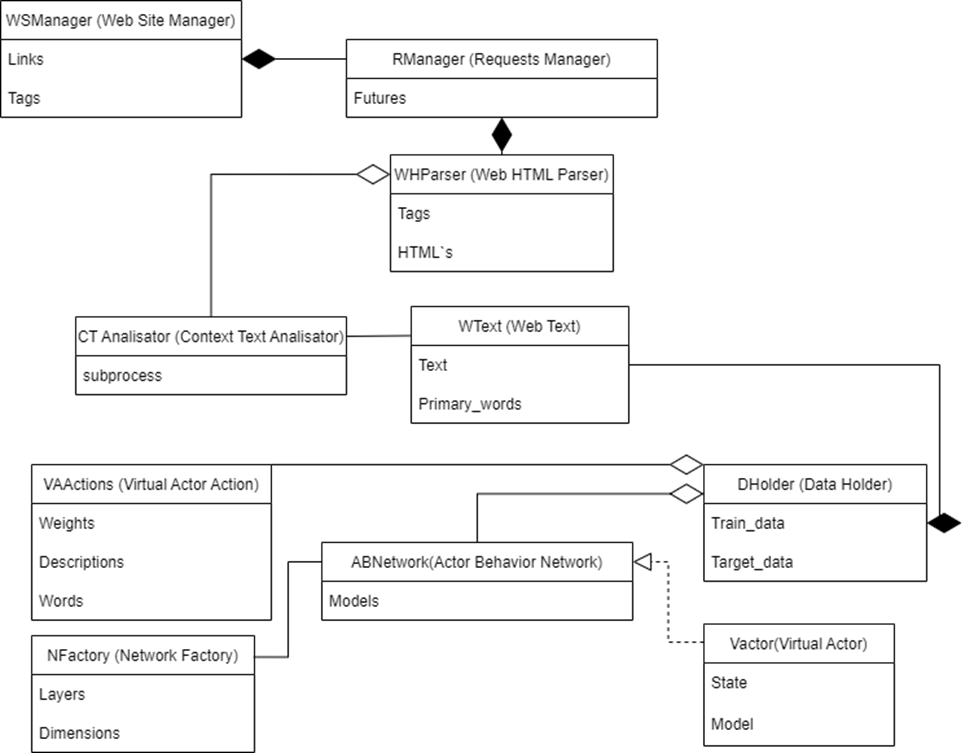
\includegraphics[width=0.75\columnwidth]{./img/ris12.png}
\centering
\caption{Связь между акторами и объектами}
\label{pic:ris12}
\end{figure}

\begin{enumerate}
  \item	В Web Site Manager попадают ссылки на все сайты, каждому сайту указываются теги.
  \item	Далее Web Site Manager передает ссылки в Request Manager.
  \item	Request Manager асинхронно посылает запросы на сайт, чтобы получить весь контент сайта, по запросу он получает html-страницу и передает ее в Web Html Parser.
  \item	Web Html Parser по тегам парсит html так, что выделяет нужный текст, который передается в Web Text.
  \item	Context Text Analisator -  использует консольное приложение по работе с LingvoNET, с которым класс общается посредством стандартного ввода/вывода с целью классификации текста на предмет семантической принадлежности.
  \item	В Web Text выделяются ключевые слова при помощи Virtual Actor Action.
  \item	Virtual Actor Action берутся из excel-таблицы действий со значением весов и описаниями.
  \item	В Data Holder на основании Virtual Actor Action и самого текста генерируются сценарии (10 действий, 11 состояний), моделью пытаемся предсказать 11 состояние на основе 10 предыдущих.
  \item	Actor Behavior Network хранит все обученные модели, из которых потом выбирается оптимальная.
  \item	Network Factory – шаблон проектирования, создает по описанию нейронной сети создает экземпляр сети (Actor Behavior Network).
  \item	Одному Virtual Actor соответствует одна нейронная сеть, у Virtual Actor меняется текущее состояние на основе модели. 
\end{enumerate}

\section{Выводы}

В процессе работы были выделены часто используемые инструменты для сбора данных со сторонних веб-сервисов, 
а именно программные модули языка Python requests, Asyncio, ButifulSoup. 
Произведен анализ инструментария для решения задач семантической близости слов. 
Также была составлена диаграмма классов программного модуля. 
А для моделирования поведения виртуального агента составлена архитектура рекуррентной нейронной сети.



